As discussed previously, the ambisonics signals provide a valid description of the captured sound field only in a spherical region around the ambisonics microphone that extends up to the nearest source or obstacle.
Consequently, in order to determine the set of microphones for which the listening position is valid, we must first locate any near-field sources.
Several existing methods for acoustically localizing near-field sources using ambisonics signals from one or more ambisonics microphones are discussed by~\citet[chapter 3]{Zheng2013PhD}, and require only knowledge of the positions and orientations of the microphones.%\footnote{Note that in the present method, we only aim to determine the locations of sources, whereas \citet{Zheng2013PhD} additionally attempts to isolate their emitted signals.}

Briefly, such methods often involve taking a short-time Fourier transform of the first-order ambisonics signals and, for each time-frequency bin, calculating the acoustic intensity vector, as given in \eqnref{eq:04_Auditory_Models:Intensity_Vector}. % \citet[Eq.~(11)]{MerimaaPulkki2005}.
For each ambisonics microphone, a histogram is generated using the direction of the intensity vector at each time and frequency.
The peaks of the histogram indicate source directions, and source positions are determined through triangulation with multiple ambisonics microphones.

Once the locations of the near-field sources are determined, we compare the distances from each microphone to its nearest source and the distance of that microphone to the desired listening position.
Only the signals from those microphones that are nearer to the listening position than to any near-field source are included in the navigation calculation (i.e., all microphones such that $r_p = \|\vec{r}_0 - \vec{u}_p\| < \|\vec{s}_0 - \vec{u}_p\| = s_p$).
A matrix of interpolation filters, described in the following sections, is then computed for and applied to the signals from the remaining ``valid'' microphones.
This procedure is illustrated by the flowchart in \figref{fig:08_Proposed_Method:Flowchart}.

% Flowchart
\begin{figure*}[t]
    \centering
    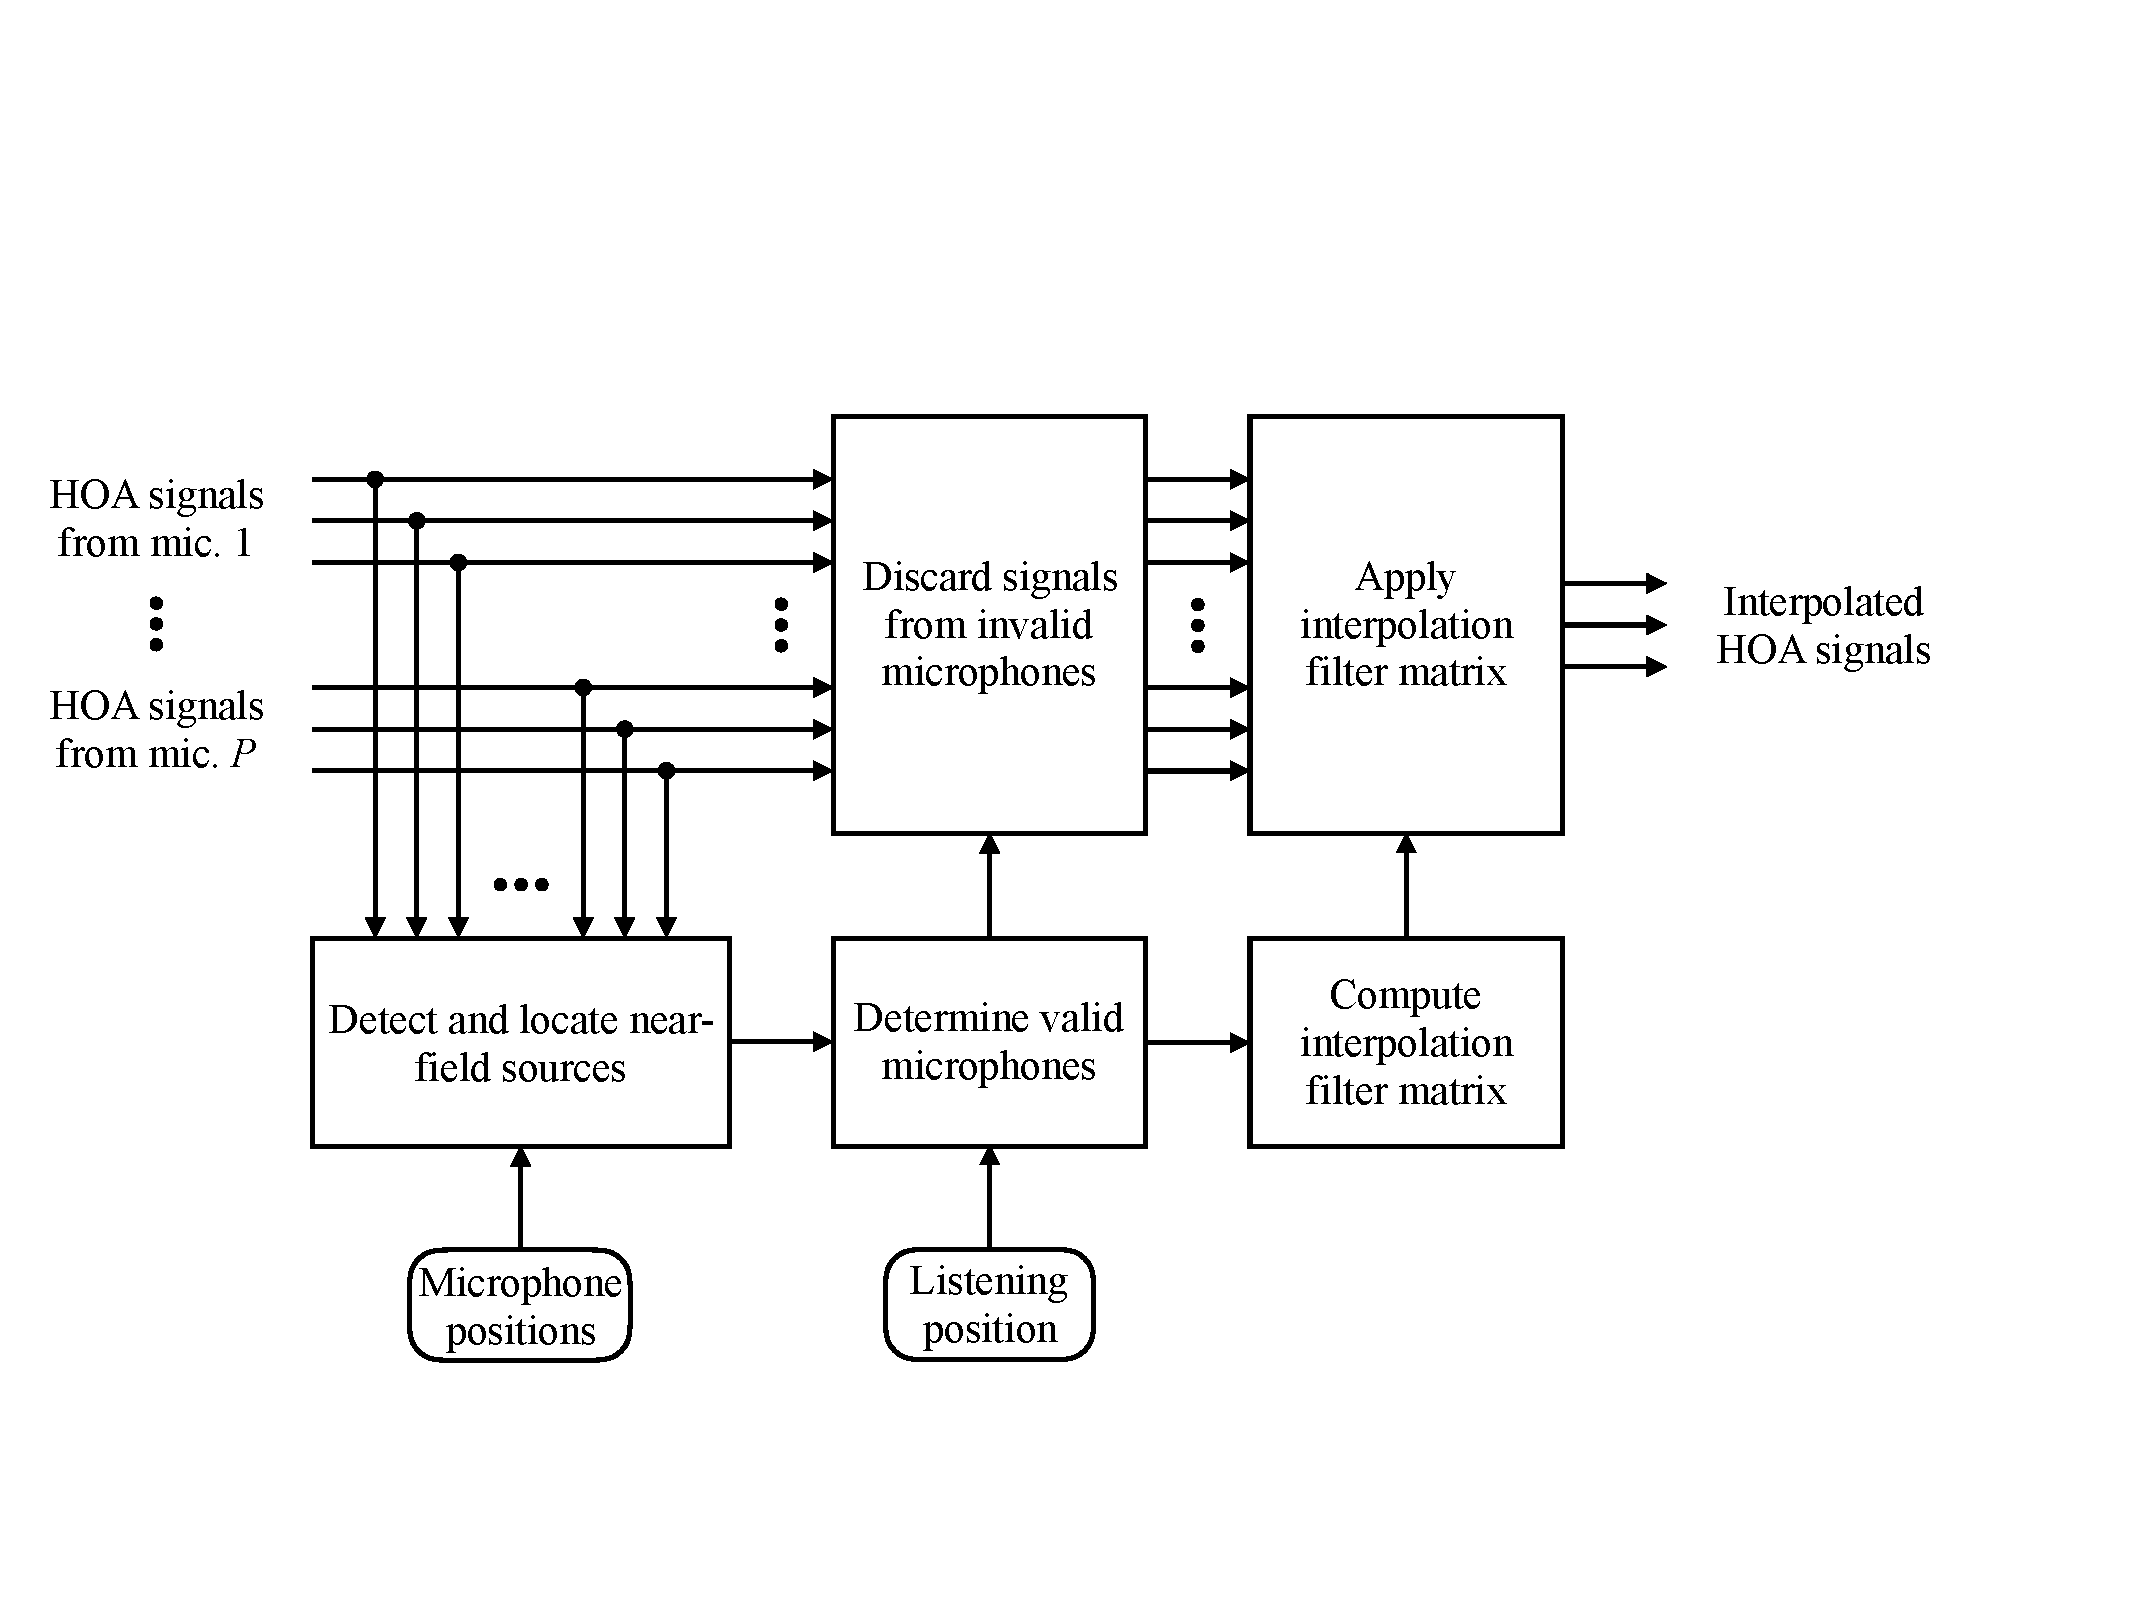
\includegraphics[width = \textwidth,trim={0 4cm 3cm 7cm},clip]{08_proposed_method/figures/Interpolation_Flowchart.pdf}
\caption[Flowchart of the proposed parametric interpolation method.]{
Flowchart of the proposed method for virtual sound field navigation excluding invalid microphones.}
\label{fig:08_Proposed_Method:Flowchart}
\end{figure*}
%%NOTE%% convert to tikz

In this work, we assume that any near-field sound sources can be located accurately and we choose to focus on characterizing the performance of the proposed navigational method under that assumption.
Accordingly, we do not concern ourselves with the sensitivity of the proposed method to inaccuracies in the estimated positions of near-field sources.
This assumption will be valid in scenarios where the positions of the nearest sound sources are either known \textit{a priori} or can be accurately obtained (e.g., through physical distance measurements) \textit{a posteriori}.